\documentclass[10pt]{article}
\usepackage[a4paper,margin=0.65in]{geometry}
\usepackage{amsmath,amssymb,graphicx,booktabs,array,float,hyperref,enumitem,xcolor,tikz}
\usetikzlibrary{positioning,arrows.meta,shapes.geometric,fit,calc}
\setlist{nosep,leftmargin=*}
\renewcommand{\arraystretch}{1.12}
\setlength{\parindent}{0pt}
\setlength{\parskip}{2pt}
\graphicspath{{lab8_figures/}}
\begin{document}
\begin{center}
{\large\textbf{Shiv Nadar University Chennai}}\\[2mm]
{\normalsize\textbf{CS3807 -- Deep Learning Laboratory}}\\[2mm]
{\large\textbf{Experiment 8}}\\[1mm]
{\normalsize\textbf{Attention Mechanisms in ResNet50 for Flower Image Classification}}
\end{center}
\vspace{3mm}
\begin{tabular}{|p{3.4cm}|p{9.0cm}|p{1.4cm}|}\hline
Degree \& Branch & B.Tech Artificial Intelligence \& Data Science & Semester V\\\hline
Subject Code \& Name & CS3807 -- Deep Learning Laboratory & AY: 2026--27\\\hline
\end{tabular}

\section*{1. Objective}
The objective is to implement and compare attention mechanisms within an ImageNet-pretrained ResNet50 classifier for five-class flower recognition. The study examines attention type, insertion stage, multiple insertion positions, channel/spatial order, spatial-attention kernel size, and additional mechanisms. Performance is assessed using classification metrics, model complexity, inference latency, training curves, confusion matrices, and qualitative visualizations.

\section*{2. Learning Outcomes}
The experiment studies: (i) channel, spatial, self, combined, SE, ECA and CBAM attention; (ii) stage-wise attention placement; (iii) the effect of applying attention at multiple stages; (iv) channel--spatial ordering; (v) spatial-kernel size; (vi) transfer learning and fine-tuning; (vii) accuracy, precision, recall, macro F1 and confusion-matrix analysis; and (viii) the accuracy--complexity and F1--latency trade-offs.

\section*{3. Dataset and Experimental Setup}
\textbf{Dataset: TensorFlow Flowers (`tf\_flowers`).} The task is five-class image classification with the classes dandelion, daisy, tulips, sunflowers and roses. The notebook resizes images to $224\times224$ pixels and uses the ResNet50 preprocessing pipeline. The data split is 70\% training, 15\% validation and 15\% testing. The recorded test set contains 550 images. A fixed seed of 42 is used in the notebook.
\begin{center}
\begin{tabular}{|l|l|}\hline
Backbone & ResNet50, ImageNet-pretrained\\\hline
Input size & $224\times224\times3$\\\hline
Batch size & 8\\\hline
Feature-extraction epochs & 3\\\hline
Fine-tuning epochs & 2\\\hline
Dropout & 0.3\\\hline
Feature-extraction learning rate & $10^{-3}$\\\hline
Fine-tuning learning rate & As configured in notebook\\\hline
Loss & Categorical cross-entropy\\\hline
Test images & 550\\\hline
\end{tabular}
\end{center}
The epoch counts are the values used in this run; they are not presented as mandatory defaults from the manual. The same split and common training procedure are used for comparisons where applicable.

\begin{figure}[H]\centering\includegraphics[width=0.90\textwidth]{dataset_examples.png}\caption{Example images from the dataset.}\end{figure}
\begin{figure}[H]\centering\includegraphics[width=0.88\textwidth]{class_distribution.png}\caption{Class distribution recorded by the notebook.}\end{figure}

\section*{4. Model and Attention Overview}
ResNet50 extracts progressively higher-level features through residual stages. Attention blocks reweight feature channels, spatial positions, or relationships between spatial locations. Channel attention learns which feature channels are useful; spatial attention learns where informative features occur; self-attention models interactions between positions; SE and ECA are channel-focused mechanisms; CBAM combines channel and spatial attention.
\begin{center}
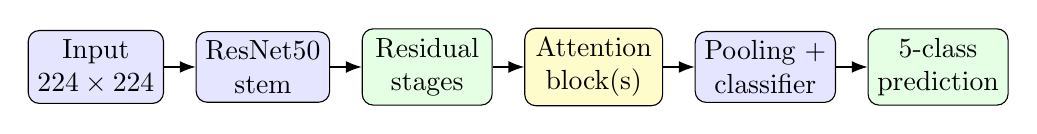
\begin{tikzpicture}[node distance=4mm]
\node[draw,rounded corners,fill=blue!10,align=center,minimum width=1.65cm,minimum height=0.65cm](a){Input\\$224\times224$};
\node[draw,rounded corners,fill=blue!10,align=center,right=of a,minimum width=1.65cm,minimum height=0.65cm](b){ResNet50\\stem};
\node[draw,rounded corners,fill=green!10,align=center,right=of b,minimum width=1.65cm,minimum height=0.65cm](c){Residual\\stages};
\node[draw,rounded corners,fill=yellow!20,align=center,right=of c,minimum width=1.75cm,minimum height=0.65cm](d){Attention\\block(s)};
\node[draw,rounded corners,fill=blue!10,align=center,right=of d,minimum width=1.65cm,minimum height=0.65cm](e){Pooling +\\classifier};
\node[draw,rounded corners,fill=green!10,align=center,right=of e,minimum width=1.45cm,minimum height=0.65cm](f){5-class\\prediction};
\foreach \x/\y in {a/b,b/c,c/d,d/e,e/f}\draw[-{Latex[length=2mm]}](\x)--(\y);
\end{tikzpicture}
\end{center}

\section*{5. Training Curves}
The notebook records three feature-extraction epochs followed by two fine-tuning epochs. The curves below are taken from the executed notebook outputs. They show the evolution of training and validation metrics; short runs mean the curves should be interpreted as evidence of this run only, not as a full convergence study.
\subsection*{5.1 Baseline ResNet50}
\begin{figure}[H]\centering\includegraphics[width=0.78\textwidth]{baseline_feature_accuracy.png}\caption{Baseline feature-extraction accuracy.}\end{figure}
\begin{figure}[H]\centering\includegraphics[width=0.78\textwidth]{baseline_feature_loss.png}\caption{Baseline feature-extraction loss.}\end{figure}
\begin{figure}[H]\centering\includegraphics[width=0.78\textwidth]{baseline_finetune_accuracy.png}\caption{Baseline fine-tuning accuracy.}\end{figure}
\begin{figure}[H]\centering\includegraphics[width=0.78\textwidth]{baseline_finetune_loss.png}\caption{Baseline fine-tuning loss.}\end{figure}
\subsection*{5.2 Manual Experiment 2: Attention after conv4\_x}
\begin{figure}[H]\centering\includegraphics[width=0.78\textwidth]{b3_feature_accuracy.png}\caption{Feature-extraction accuracy for channel--spatial attention after conv4\_x.}\end{figure}
\begin{figure}[H]\centering\includegraphics[width=0.78\textwidth]{b3_feature_loss.png}\caption{Feature-extraction loss for channel--spatial attention after conv4\_x.}\end{figure}
\begin{figure}[H]\centering\includegraphics[width=0.78\textwidth]{b3_finetune_accuracy.png}\caption{Fine-tuning accuracy for channel--spatial attention after conv4\_x.}\end{figure}
\begin{figure}[H]\centering\includegraphics[width=0.78\textwidth]{b3_finetune_loss.png}\caption{Fine-tuning loss for channel--spatial attention after conv4\_x.}\end{figure}

\section*{6. Main Experimental Results}
The experiment headings below follow the Lab 8 manual's experiment numbering (manual Sections 14--19).
\subsection*{Experiment 1 (Manual Section 14): Attention-Type Ablation}
The baseline was compared with channel, spatial, channel--spatial, self-attention and combined attention at P3 (after conv4\_x). The baseline and spatial-attention P3 models both recorded 93.28\% final validation accuracy. The complete per-model results are provided in Section 7 so that lower-performing variants are also represented. The experiment demonstrates that adding an attention module does not guarantee a higher score under a fixed short training budget.

\subsection*{Experiment 2 (Manual Section 15): Attention-Position Ablation}
The same channel--spatial attention design was trained after conv2\_x, conv3\_x, conv4\_x and conv5\_x. The feature resolutions/channels specified by the manual are 56$\times$56/256, 28$\times$28/512, 14$\times$14/1024 and 7$\times$7/2048, respectively. The recorded validation accuracies for the manual-aligned variants were 89.29\% (conv2\_x), 90.93\% (conv3\_x), 92.20\% (conv4\_x) and 92.92\% (conv5\_x). On the held-out test set, the conv4\_x variant obtained 93.27\% accuracy and macro F1 of 93.29\%, the highest test accuracy among the evaluated variants in the recorded table. These results are specific to this run.

\subsection*{Experiment 3 (Manual Section 16): Multiple Attention Positions}
The notebook compares attention at P3 only, P4 only and P3+P4. Their recorded final validation accuracies are shown in the all-experiment table. The purpose is to test whether repeated attention yields enough predictive improvement to justify extra parameters and computation. In this run, P3+P4 does not outperform the best single-position configurations on validation or test metrics.

\subsection*{Experiment 4 (Manual Section 17): Attention Order}
D1 applies channel attention followed by spatial attention; D2 reverses the order. D2 reaches 92.92\% final validation accuracy and 92.91\% test accuracy, while D1 reaches 92.20\% final validation accuracy and 91.27\% test accuracy. Under this run's settings, spatial--channel ordering performed better, although repeated seeds would be needed to establish whether the difference is robust.

\subsection*{Experiment 5 (Manual Section 18): Spatial-Attention Kernel Size}
Spatial attention with 3$\times$3, 5$\times$5 and 7$\times$7 kernels was evaluated at P3. Their recorded final validation accuracies were 90.56\%, 92.01\% and 92.01\%, respectively. The 5$\times$5 and 7$\times$7 variants were close in validation accuracy; the held-out test table should be considered separately rather than assuming the best validation result also has the best test result.

\subsection*{Additional Task (Manual Section 19): Additional Attention Mechanisms}
The notebook includes SE, ECA and CBAM at P3, satisfying the requirement to compare at least two additional mechanisms. Their test metrics, model parameters and latency are listed in Section 7. SE is competitive with the baseline, while ECA and CBAM show slightly lower recorded test accuracy in this run. The differences are small and should not be generalized beyond the single experimental run.

\section*{7. Quantitative Comparison}
Table~\ref{tab:allresults} combines validation accuracy, held-out test accuracy, test macro precision, recall and macro F1, total parameters and recorded inference latency. The test metrics are generated from the notebook's report-ready comparison cell. Missing values are not imputed.
\begin{table}[H]\centering\scriptsize\setlength{\tabcolsep}{2pt}
\resizebox{\textwidth}{!}{%
\begin{tabular}{p{3.3cm}rrrrrrr}
\toprule
Experiment & Val. acc. (\%) & Test acc. (\%) & Precision (\%) & Recall (\%) & Macro F1 (\%) & Parameters & ms/image\\
\midrule
A0 Baseline & 93.28 & 92.36 & 92.57 & 92.47 & 92.50 & 23597957 & 29.91 \\
A2 Spatial P3 & 93.28 & 91.64 & 91.93 & 91.62 & 91.74 & 23598055 & 29.44 \\
A3 Channel+Spatial P3 & 93.10 & 91.64 & 91.87 & 91.81 & 91.81 & 23730215 & 30.20 \\
A5 Combined P3 & 92.92 & 92.91 & 93.05 & 93.00 & 93.01 & 24254503 & 30.37 \\
D2 Spatial-to-Channel & 92.92 & 92.91 & 93.45 & 92.79 & 93.01 & 23730215 & 29.66 \\
E Kernel 7x7 & 92.92 & 92.18 & 92.13 & 92.48 & 92.24 & 23598055 & 29.17 \\
Exp.2 B4 after conv5\_x & 92.92 & 91.82 & 91.94 & 91.72 & 91.76 & 24124519 & 29.58 \\
C2 P4 only & 92.74 & 92.73 & 92.88 & 92.69 & 92.74 & 24124519 & 29.67 \\
C1 P3 only & 92.74 & 92.55 & 92.77 & 92.71 & 92.70 & 23730215 & 29.51 \\
A1 Channel P3 & 92.56 & 92.36 & 92.53 & 92.40 & 92.46 & 23730117 & 29.67 \\
A6 SE P3 & 92.56 & 92.36 & 92.68 & 92.28 & 92.39 & 23730117 & 29.77 \\
Exp.2 B3 after conv4\_x & 92.20 & 93.27 & 93.19 & 93.40 & 93.29 & 23730215 & 29.42 \\
B1 Channel+Spatial P2 & 92.20 & 90.91 & 91.05 & 91.06 & 91.02 & 23631367 & 29.77 \\
D1 Channel-to-Spatial & 92.20 & 91.27 & 91.56 & 91.31 & 91.38 & 23730215 & 29.83 \\
A7 ECA P3 & 92.01 & 92.00 & 91.90 & 92.06 & 91.95 & 23597960 & 29.92 \\
E Kernel 5x5 & 92.01 & 92.36 & 92.43 & 92.42 & 92.41 & 23598007 & 29.34 \\
C3 P3+P4 & 92.01 & 91.64 & 91.72 & 91.72 & 91.70 & 24256777 & 30.55 \\
B2 Channel+Spatial P3 & 91.65 & 92.18 & 92.55 & 92.12 & 92.28 & 23730215 & 30.04 \\
A8 CBAM P3 & 90.93 & 91.82 & 91.95 & 91.91 & 91.92 & 23730215 & 29.86 \\
Exp.2 B2 after conv3\_x & 90.93 & 90.73 & 91.12 & 90.98 & 91.00 & 23631367 & 29.54 \\
E Kernel 3x3 & 90.56 & 90.55 & 90.70 & 90.54 & 90.58 & 23597975 & 29.37 \\
A4 Self-attention P3 & 90.38 & 90.36 & 90.50 & 90.67 & 90.53 & 24122245 & 29.74 \\
Exp.2 B1 after conv2\_x & 89.29 & 87.45 & 87.59 & 87.63 & 87.59 & 23606519 & 29.82 \\
\bottomrule
\end{tabular}}
\caption{Recorded validation and held-out test results. Latency is environment-dependent.}\label{tab:allresults}
\end{table}

The highest held-out test accuracy in the executed comparison is Exp.2 B3 after conv4\_x at 93.27\%, with macro F1 93.29\%. The baseline test accuracy is 92.36\%. The selected model variable in the notebook's earlier evaluation cell resolved to A0\_Baseline; therefore, the report does not treat the baseline confusion matrix as a confusion matrix for the highest-test-accuracy model. This distinction is retained to avoid mislabelling an output.

\begin{figure}[H]\centering\includegraphics[width=\textwidth]{validation_accuracy_comparison.png}\caption{Fine-tuning validation-accuracy comparison across completed experiments.}\end{figure}
\begin{figure}[H]\centering\includegraphics[width=\textwidth]{inference_time_comparison.png}\caption{Recorded inference-time comparison across experiments.}\end{figure}
\begin{figure}[H]\centering\includegraphics[width=0.92\textwidth]{accuracy_complexity.png}\caption{Accuracy--model-complexity trade-off.}\end{figure}
\begin{figure}[H]\centering\includegraphics[width=0.92\textwidth]{macro_f1_latency.png}\caption{Macro-F1 versus inference-latency trade-off.}\end{figure}

\section*{8. Confusion Matrix and Class-wise Analysis}
The executed notebook contains a baseline confusion matrix and a class-wise classification report for the model referenced by its evaluation cell. Because that cell's selected-model name resolved to A0\_Baseline, the class-wise metrics below are reported as baseline metrics rather than being attributed to the highest-test-accuracy B3 manual-position model.
\begin{figure}[H]\centering\includegraphics[width=0.78\textwidth]{confusion_baseline.png}\caption{Confusion matrix for the baseline ResNet50.}\end{figure}
\begin{center}\begin{tabular}{lrrrr}\toprule
Class & Precision & Recall & F1-score & Support\\\midrule
Dandelion & 0.95 & 0.97 & 0.96 & 112\\
Daisy & 0.97 & 0.94 & 0.95 & 95\\
Tulips & 0.90 & 0.90 & 0.90 & 134\\
Sunflowers & 0.91 & 0.94 & 0.93 & 102\\
Roses & 0.90 & 0.87 & 0.89 & 107\\\bottomrule
\end{tabular}\end{center}
The baseline report shows the lowest recall for roses (0.87), while dandelions have the highest recall (0.97). A confusion matrix reveals which classes are confused with each other, information that a single accuracy score cannot provide.

\section*{9. Attention and Feature Visualizations}
\subsection*{9.1 Feature Maps Before and After Attention}
\begin{figure}[H]\centering\includegraphics[width=0.90\textwidth]{feature_maps_before_after.png}\caption{Feature-map response before and after channel attention.}\end{figure}
\subsection*{9.2 Channel Attention}
\begin{figure}[H]\centering\includegraphics[width=0.95\textwidth]{channel_attention_weights.png}\caption{Channel-attention weights.}\end{figure}
\subsection*{9.3 Spatial Attention}
\begin{figure}[H]\centering\includegraphics[width=\textwidth]{spatial_attention_heatmap_overlay.png}\caption{Spatial-attention map and overlay.}\end{figure}
\subsection*{9.4 Self-Attention Response}
\begin{figure}[H]\centering\includegraphics[width=0.72\textwidth]{self_attention_response.png}\caption{Self-attention response.}\end{figure}
\subsection*{9.5 Grad-CAM}
\begin{figure}[H]\centering\includegraphics[width=\textwidth]{gradcam_baseline_channel.png}\caption{Baseline and channel-attention Grad-CAM comparison.}\end{figure}
Grad-CAM is a post-hoc visualization of class-score gradients with respect to convolutional feature maps. It is distinct from an internal attention map and should be interpreted as a qualitative explanation rather than proof of causal importance.
\subsection*{9.6 Attention Position: P2, P3 and P4}
\begin{figure}[H]\centering\includegraphics[width=\textwidth]{attention_positions_p2_p3_p4.png}\caption{Attention maps at P2, P3 and P4.}\end{figure}

\section*{10. Qualitative Error Inspection}
The notebook produced a five-image comparison with three correctly classified and two incorrectly classified examples. However, because the selected-model variable resolved to the baseline, the executed comparison used the baseline as both comparison targets. This figure is therefore included only as an example-selection record and is not used to claim that attention improves localization or error handling.
\begin{figure}[H]\centering\includegraphics[width=0.72\textwidth]{qualitative_3correct_2incorrect.png}\caption{Three correct and two incorrect examples recorded by the notebook. The comparison target resolves to the baseline in this execution.}\end{figure}
A valid across-mechanism qualitative conclusion requires rerunning the evaluation-only cell after explicitly selecting the intended attention model and its matching attention map and weights. This is an evaluation fix, not a need to retrain models.

\section*{11. Discussion}
The experiments show that the effect of attention depends on its type and insertion point. The manual-aligned conv4\_x channel--spatial model has the highest observed held-out test accuracy (93.27\%) and macro F1 (93.29\%) in the recorded comparison. D2 spatial--channel ordering is also competitive. Multiple attention positions do not automatically improve results, and additional parameter count alone is not a reliable indicator of predictive quality. The inference-time measurements are clustered around approximately 29--31 ms per image in this runtime; such measurements depend on hardware, warm-up and batch/synchronization conditions.

The main limitations are the short training schedule (three feature-extraction epochs and two fine-tuning epochs), a single recorded run, environment-dependent inference timing, and the selected-model variable mismatch in the qualitative/confusion-matrix evaluation. Attention maps and Grad-CAM are qualitative aids; they do not independently establish causal explanations. The report therefore separates recorded validation results from held-out test metrics and does not attribute baseline-only plots to a different model.

\section*{12. Conclusion}
This experiment implemented a ResNet50 transfer-learning pipeline and compared attention type, position, multiple positions, channel--spatial order, kernel size, and SE/ECA/CBAM mechanisms on five flower classes. Across the evaluated models, channel--spatial attention after conv4\_x achieved the highest recorded test accuracy of 93.27\% and macro F1 of 93.29\%. The baseline achieved 92.36\% test accuracy, showing a modest improvement for the strongest test-scoring variant in this run. Further repeated-seed experiments and a corrected evaluation-only selection cell are recommended before making strong general claims.

\section*{13. References}
\begin{enumerate}
\item K. He, X. Zhang, S. Ren and J. Sun, ``Deep Residual Learning for Image Recognition,'' CVPR, 2016.
\item J. Hu, L. Shen and G. Sun, ``Squeeze-and-Excitation Networks,'' CVPR, 2018.
\item S. Woo et al., ``CBAM: Convolutional Block Attention Module,'' ECCV, 2018.
\item Q. Wang et al., ``ECA-Net: Efficient Channel Attention for Deep Convolutional Neural Networks,'' CVPR, 2020.
\item TensorFlow Datasets, ``tf\_flowers,'' \url{https://www.tensorflow.org/datasets/catalog/tf_flowers}.
\item TensorFlow/Keras Applications, ResNet50 documentation, \url{https://keras.io/api/applications/resnet/}.
\end{enumerate}

\vspace{4mm}
\textbf{Name:} T Pranav Varshin (24110413)\\
\textbf{Reg. No.:} 24011101116\\
\textbf{Section:} AIDS-B
\end{document}
